%%%%%%%%%%%%%%%%%%%%%%%%%%%%%%%%%%%%%%%%%%%%%%%%%%%%%%%%%%%%%%%%%%%%%
%
% Complete documentation on the extended LaTeX markup used for Insight
% documentation is available in ``Documenting Insight'', that is part
% of the standard documentation for Insight.  It may be found online
% at:
%
%                    http://www.itk.org
%
%%%%%%%%%%%%%%%%%%%%%%%%%%%%%%%%%%%%%%%%%%%%%%%%%%%%%%%%%%%%%%%%%%%%%

\documentclass{InsightSoftwareGuide}


\usepackage[dvips]{graphicx}
\usepackage{times,lscape,url}
%\usepackage{mdwtab}


%%% \usepackage[latin1]{inputenc}
%%% \selectlanguage{french}
% Configuration pour les accents francais pour l'OTB
\usepackage[latin1]{inputenc}
%\usepackage[french]{babel}
\usepackage{tikz}


\usepackage{color}

\definecolor{listcomment}{rgb}{0.0,0.5,0.0}
\definecolor{listkeyword}{rgb}{0.0,0.0,0.5}
\definecolor{listnumbers}{gray}{0.65}
\definecolor{listlightgray}{gray}{0.955}
\definecolor{listwhite}{gray}{1.0}

\usepackage{listings}
\newcommand{\lstsetcpp}
{
\lstset{frame = tb,
       framerule = 0.25pt,
       float,
       fontadjust,
       backgroundcolor={\color{listlightgray}},
       basicstyle = {\ttfamily\footnotesize},
       keywordstyle = {\ttfamily\color{listkeyword}\textbf},
       identifierstyle = {\ttfamily},
       commentstyle = {\ttfamily\color{listcomment}\textit},
       stringstyle = {\ttfamily},
       showstringspaces = false,
       showtabs = false,
       numbers = none,
       numbersep = 6pt,
       numberstyle={\ttfamily\color{listnumbers}},
       tabsize = 2,
       language=[ANSI]C++,
       floatplacement=!h
       }
}
\newcommand{\lstsetpython}
{
\lstset{language=Python
        }
}
\newcommand{\lstsetjava}
{
\lstset{language=Java
        }
}


\newif\ifitkFullVersion
\itkFullVersiontrue
%\itkFullVersionfalse

\newif\ifitkPrintedVersion
\itkPrintedVersiontrue
%\itkPrintedVersionfalse


%%%%%%%%%%%%%%%%%%%%%%%%%%%%%%%%%%%%%%%%%%%%%%%%%%%%%%%%%%%%%%%%%%
%
%  hyperref should be the last package to be loaded.
%
%%%%%%%%%%%%%%%%%%%%%%%%%%%%%%%%%%%%%%%%%%%%%%%%%%%%%%%%%%%%%%%%%%
\ifitkPrintedVersion
\usepackage[dvips,
pdftitle={Monteverdi Guide},
pdfauthor={CNES},
pdfsubject={Remote Sensing, Orfeo, Pleiades, Cosmo Skymed},
pdfkeywords={image processing, Remote sensing, Guide},
pdfpagemode={UseOutlines},
bookmarks,bookmarksopen,
pdfstartview={FitH},
backref,
colorlinks,linkcolor={black},citecolor={black},urlcolor={black},
]{hyperref}
\else
\usepackage[dvips,
pdftitle={Monteverdi Guide},
pdfauthor={CNES},
pdfsubject={Remote Sensing, Orfeo, Pleiades, Cosmo Skymed},
pdfkeywords={image processing, Remote sensing, Guide},
pdfpagemode={UseOutlines},
bookmarks,bookmarksopen,
pdfstartview={FitH},
backref,
colorlinks,linkcolor={blue},citecolor={blue},urlcolor={blue},
]{hyperref}
\fi

\usepackage{amsmath,amssymb,amsfonts}
\usepackage{bbm}
%%%%%%%%%%%%%%%%%%%%%%%%%%%%%%%%%%%%%%%%%%%%%%%%%%%%%%%%%%%%%%%%%%%
%
%
%   Load configuration parameters prepared by CMake
%
%
%%%%%%%%%%%%%%%%%%%%%%%%%%%%%%%%%%%%%%%%%%%%%%%%%%%%%%%%%%%%%%%%%%%

% Define where in the disk is the Insight source tree 
% \def\ITKSOURCEDIR{}
% THOMAS
\def\ITKSOURCEDIR{/ORFEO/thomas/ORFEO-TOOLBOX/otb/OTB}
\graphicspath{{/ORFEO/thomas/ORFEO-TOOLBOX/otb/OTB-Documents/SoftwareGuide/Art/}{/ORFEO/thomas/ORFEO-TOOLBOX/otb/OTB-Documents/SoftwareGuide/Art/}}
\def\bibtexdatabasepath{/ORFEO/thomas/ORFEO-TOOLBOX/otb/OTB-Documents/SoftwareGuide/../Latex/Insight}


% Define command to make reference to on-line Doxygen documentation
\newcommand{\doxygen}[1]{
\href{http://www.itk.org/Doxygen/html/classitk_1_1#1.html}{\code{itk::#1}}}  

% Define command to make reference to on-line Doxygen documentation
\newcommand{\subdoxygen}[2]{
\href{http://www.itk.org/Doxygen/html/classitk_1_1#1_1_1#2.html}{\code{itk::#1::#2}}}  

% Define command for the standard comment introducing classes with similar functionalities
\newcommand{\relatedClasses}{
\textbf{The following classes provide similar functionality:}}


\def\logoCNES{CNES_nom.eps}

\newtheorem{algo}{Algorithm}
\newtheorem{defin}{Definition}
%%%%%%%%%%%%%%%%%%%%%%%%%%%%%%%%%%%%%%%%%%%%%%%%%%%%%%%%%%%%%%%%%%%
%
%
%           The Insight Toolkit Software Guide
%
%
%%%%%%%%%%%%%%%%%%%%%%%%%%%%%%%%%%%%%%%%%%%%%%%%%%%%%%%%%%%%%%%%%%%

\title{The Monteverdi Guide\\ Updated
  for OTB-3.2}

\author{OTB Development Team}

\authoraddress{
  \url{http://www.orfeo-toolbox.org}\\
  e-mail: \email{otb@cnes.fr}
}

\date{\today}


% actually write the .idx file
\makeindex

\setcounter{tocdepth}{3}



%%%%%%%%%%%%%%%%%%%%%%%%%%%%%%%%%%%%%%%%%%%%%%%%%%%%%%%%%%%%%%%%%%%
%
%           Begin Document
%
%%%%%%%%%%%%%%%%%%%%%%%%%%%%%%%%%%%%%%%%%%%%%%%%%%%%%%%%%%%%%%%%%%%

\begin{document}

\ifitkPrintedVersion
%% 
\begin{minipage}[t][3cm][b]{\textwidth}
\rule{14cm}{1pt}
\end{minipage}


\begin{minipage}[t][3cm][b]{\textwidth}
\Huge
The ITK Software Guide\\
\normalsize
\par
\emph{updated for version 2.4}\\
\end{minipage}

\hfill
\begin{minipage}[t][6cm][b]{0.6\textwidth}
\Large
\renewcommand{\baselinestretch}{1.5}
Luis Ib\'{a}\~{n}ez\\
Will Schroeder\\
Lydia Ng\\
Josh Cates\\
and the \emph{Insight Software Consortium}
\normalsize
\end{minipage}


\begin{minipage}[t][2cm][b]{\textwidth}
\rule{14cm}{1pt}
\end{minipage}

\newpage

\begin{minipage}[t][4cm][b]{\textwidth}
\begin{center}

\includegraphics[width=0.5\textwidth]{Kitware-logo-medium-res.eps}
\end{center}
\par
\begin{center}
\large
\copyright 2003 Kitware, Inc. \emph{(cover, preface, postface)}\\
\copyright 2003 Insight Software Consortium \emph{(main text body)}\\
Published by Kitware, Inc. \texttt{http://www.kitware.com}
\normalsize
\end{center}
\end{minipage}


\begin{minipage}[t][2.25cm][b]{\textwidth}
\begin{center}
All rights reserved. No part of this book may be reproduced, in any form 
or by any means, without the express written permission of the copyright
holders. An electronic version of this document is available from
\texttt{http://www.itk.org} and may be used under the provisions of the
ITK copyright found at \texttt{http://www.itk.org/HTML/Copyright.htm}.
\end{center}
\end{minipage}


\begin{minipage}[t][3.2cm][b]{\textwidth}
\begin{center}
The publisher Kitware, Inc. offers discounts on this book when ordered in
bulk quantities.\\
The publisher also produces companion works to this text such as \emph{The
Visualization Toolkit An Object-Oriented Approach to 3D Graphics 3rd Edition}
by Schroeder, Martin and Lorensen, \emph{Mastering CMake} by Martin and
Hoffman and \emph{The VTK's Users Guide} by Kitware.\\
For more information contact Kitware, Inc at \texttt{kitware@kitware.com}.\\
You may also order directly from Kitware's electronic store at
\texttt{http://www.kitware.com/products}\\
\end{center}
\end{minipage}

\begin{minipage}[t][2.7cm][b]{\textwidth}
\begin{center}
Contributors to this work include those listed on the title page as well
as:\\ Cover Design: Luis Ib\'{a}\~{n}ez and S\'{e}bastien Barr\'{e}\\
Technical Contributors: World-Wide ITK Developer Community at
\texttt{www.itk.org}. \\Document created with \LaTeX{}, using CMake as
configuration manager, with a Perl script to extract examples from the
\code{Insight/Examples} directory. All code in this document compiled at
the time of publication.
\end{center}
\end{minipage}


\begin{minipage}[t][2.5cm][b]{\textwidth}
\begin{center}
This project has been funded in whole or in part with Federal funds from the
National Institutes of Health (NLM, NIDCR, NIMH, NEI, NINDS, NIDCD, NCI), the
NSF, and the DoD (TATRC) under the direction of the National Library of
Medicine, National Institutes of Health, contracts number N01-LM-9-3531,
N01-LM-9-3532, N01-LM-0-3501, N01-LM-0-3502, N01-LM-0-3503, and
N01-LM-0-3504.
\end{center}
\end{minipage}


\begin{minipage}[t][1.0cm][b]{\textwidth}
\begin{center}
All product names mentioned herein are the trademarks of their respective 
owners.
\end{center}
\end{minipage}


\begin{minipage}[t][1.0cm][b]{\textwidth}
\begin{center}
Printed and produced in the United States of America.\\
ISBN 1-930934-15-7
\end{center}
\end{minipage}

\fi

\maketitle

\frontmatter

\hyperbaseurl{http://www.orfeo-toolbox.org}

\lstsetcpp


%%%%%%%%%%%%%%%%%%%%%%%%%%%%%%%%%%%%%%%%%%
%
%  Page with OTB logo
%
%%%%%%%%%%%%%%%%%%%%%%%%%%%%%%%%%%%%%%%%%%
\cleardoublepage

\begin{minipage}[t][10cm][b]{\textwidth}
\center

\includegraphics[width=0.5\textwidth]{logoVectoriel.eps}
\large
\begin{center}
\emph{The ORFEO Toolbox is not a black box.}\\
\end{center}
\hspace{8cm} Ch.D.
\normalsize
\end{minipage}



%%%%%%%%%%%%%%%%%%%%%%%%%%%%%%%%%%%%%%%%%%%%%%
%
% remove headings from the following material
\pagestyle{plain}
%
%%%%%%%%%%%%%%%%%%%%%%%%%%%%%%%%%%%%%%%%%%%%%%



%%\ifitkPrintedVersion
%% % We want this material to fit on two pages
\small

\chapter*{About the Cover}

Creating the cover image demonstrating the capabilities of the toolkit was a
challenging task.\footnote{The source code for the cover is available from
InsightDocuments/SoftwareGuide/Cover/Source/.} Given that the origins of ITK
are with the Visible Human Project it seemed appropriate to create an image
utilizing the VHP data sets, and it was decided to use the more recently
acquired Visible Woman dataset.  Both the RGB cryosections and the CT scans
were combined in the same scene.

\begin{description}

\item [Removing the Gel.]
The body of the Visible Woman was immersed in a block of gel during the
freezing process. This gel appears as a blue material in the cryogenic data.
To remove the gel, the joint histogram of RGB values was computed. This
resulted in an 3D image of $256\times256\times256$ pixels. The histogram
image was visualized in VolView.\footnote{VolView is a commercial product
from Kitware. It supports ITK plug-ins and is available as a free viewer or
may be licensed with advanced functionality. See
http://www.kitware.com/products/volview.html for information.} The cluster
corresponding to the statistical distribution of blue values was identified
visually, and a separating plane was manually defined in RGB space. The
equation of this plane was subsequently used to discriminate pixels in the
gel from pixels in the anatomical structures. The gel pixels were zeroed out
and the RGB values on the body were preserved.

\item[The Skin.]
The skin was easy to segment once the gel was removed. A simple region
growing algorithm was used requiring seed points in the region previously
occupied by the gel and then set to zero values. An anti-aliasing filter was
applied in order to generate an image of pixel type float where the surface
was represented by the zero set. This data set was exported to VTK where a
contouring filter was used to extract the surface and introduce it in the VTK
visualization pipeline.

\item[The Brain.]
The visible part of the brain represents the surface of the gray matter.  The
brain was segmented using the vector version of the confidence connected
image filter.  This filter implements a region growing algorithm that starts
from a set of seed points and adds neighboring pixels subject to a condition
of homogeneity.

The set of sparse points obtained from the region growing algorithm was
passed through a mathematical morphology dilation in order to close holes and
then through a binary median filter. The binary median filter has the
outstanding characteristic of being very simple in implementation by applying
a sophisticated effect on the image. Qualitatively it is equivalent to a
curvature flow evolution of the iso-contours. In fact the binary median
filter as implemented in ITK is equivalent to the majority filter that
belongs to the family of voting filters classified as a subset of the
\emph{Larger than Life} cellular automata. Finally, the volume resulting from
the median filter was passed through the anti-aliasing image filter. As
before, VTK was used to extract the surface.

\item[The Neck Musculature.]
The neck musculature was not perfectly segmented. Indeed, the resulting
surface is a fusion of muscles, blood vessels and other anatomical
structures. The segmentation was performed by applying the
VectorConfidenceConnectedImageFilter to the cryogenic dataset. Approximately
60 seed points were manually selected and then passed to the filter as
input. The binary mask produced by the filter was dilated with a mathematical
morphology filter and smoothed with the BinaryMedianImageFilter. The
AntiAliasBinaryImageFilter was used at the end to reduce the pixelization
effects prior to the extraction of the iso-surface with vtkContourFilter.

\item[The Skull.]
The skull was segmented from the CT data set and registered to the cryogenic
data. The segmentation was performed by simple thresholding, which was good
enough for the cover image. As a result, most of the bone structures are
actually fused together. This includes the jaw bone and the cervical
vertebrae.

\item[The Eye.] 
The eye is charged with symbolism in this image. This is due in part because
the motivation for the toolkit is the analysis of the Visible Human data,
and in part because the name of the toolkit is \emph{Insight}.

The first step in processing the eye was to extract a sub-image of
$60\times60\times60$ pixels centered around the eyeball from the RGB
cryogenic data set. This small volume was then processed with the vector
gradient anisotropic diffusion filter in order to increase the homogeneity of
the pixels in the eyeball.

The smoothed volume was segmented using the
VectorConfidenceConnectedImageFilter using 10 seed points. The resulting
binary mask was dilated with a mathematical morphology filter with a
structuring element of radius one, then smoothed with a binary mean image
filter (equivalent to majority voting cellular automata). Finally the mask
was processed with the AntiAliasBinaryImageFilter in order to generate a
float image with the eyeball contour embedded as a zero set.

\item[Visualization.]
The visualization of the segmentation was done by passing all the binary
masks through the AntiAliasBinaryImageFilter, generating iso-contours with
VTK filters, and then setting up a VTK Tcl script. The skin surface was
clipped using the vtkClipPolyDataFilter using the implicit function
vtkCylinder. The vtkWindowToImageFilter proved to be quite useful for
generating the final high resolution rendering of the scene ($3000\times3000$
pixels).

\item[Cosmetic Postprocessing.]
We have to confess that we used Adobe Photoshop to post-process the image. In
particular, the background of the image was adjusted using Photoshop's color
selection. The overall composition of the image with the cover text and
graphics was also performed using Photoshop.

\end{description}

\normalsize

%%\fi

%\chapter*{Foreword}
\noindent


Beside the Pleiades (PHR) and Cosmo-Skymed (CSK) systems developments
forming ORFEO, the dual and bilateral system (France - Italy) for
Earth Observation, the ORFEO Accompaniment Program was set up, to
prepare, accompany and promote the use and the exploitation of the
images derived from these sensors.

The creation of a preparatory
program\footnote{http://smsc.cnes.fr/PLEIADES/A\_prog\_accomp.htm} is
needed because of:
\begin{itemize}
\item the new capabilities and performances of the ORFEO systems
  (optical and radar high resolution, access capability, data quality,
  possibility to acquire simultaneously in optic and radar),
\item the implied need of new methodological developments : new
  processing methods, or adaptation of existing methods,
\item the need to realise those new developments in very close
  cooperation with the final users for better integration of new
  products in their systems.

\end{itemize}

This program was initiated by CNES mid-2003 and will last until mid
2013.  It consists in two parts, between which it is necessary to keep
a strong interaction:
\begin{itemize}
\item A Thematic part,
\item A Methodological part.
\end{itemize}

The Thematic part covers a large range of applications (civil and
defence), and aims at specifying and validating value added products
and services required by end users. This part includes consideration
about products integration in the operational systems or processing
chains. It also includes a careful thought on intermediary structures
to be developed to help non-autonomous users. Lastly, this part aims
at raising future users awareness, through practical demonstrations
and validations.

The Methodological part objective is the definition and the
development of tools for the operational exploitation of the
submetric optic and radar images (tridimensional aspects, changes
detection, texture analysis, pattern matching, optic radar
complementarities). It is mainly based on R\&D studies and doctorate
and post-doctorate researches.

In this context, CNES\footnote{http://www.cnes.fr} decided to develop
the \emph{ORFEO ToolBox} (OTB), a set of algorithms encapsulated in a
software library. The goals of the OTB is to capitalise a methological
\textit{savoir faire} in order to adopt an incremental development
approach aiming to efficiently exploit the results obtained in the
frame of methodological R\&D studies.

All the developments are based on FLOSS (Free/Libre Open Source
Software) or existing CNES developments. OTB is distributed under the
C\'eCILL licence,
\url{http://www.cecill.info/licences/Licence_CeCILL_V2-en.html}.

OTB is implemented in C++ and is mainly based on
ITK\footnote{http://www.itk.org} (Insight Toolkit).


%% L'environnement de l'OTB est mis en place par l'outil CMake\footnote{http://www.cmake.org},
%% permettant ainsi de g\'{e}rer les proc\'{e}dures de compilation, g\'{e}n\'{e}ration et d'installation et ce quelque sois la plate forme cible.

%% Dans un souci d'homog\'{e}n\'{e}isation, l'OTB est con\c{c}ue et d\'{e}velopp\'{e}e suivant la philosophie et les principes \'{e}dict\'{e}s
%% par la biblioth\`{e}que ITK (programmation g\'{e}n\'{e}rique, m\'{e}canisme des \emph{Object Factories}, \emph{Smart pointers}, exceptions, \emph{Multi-Threading}, etc...).
%% Ces principes sont pr\'{e}sent\'{e}s dans le paragraphe \emph{3.2 Essential System Concepts} du guide ITK \url{http://www.itk.org/ItkSoftwareGuide.pdf}

%% Enfin, la m\'{e}thodologie de d\'{e}veloppement appliqu\'{e}e s'appuie sur une approche it\'{e}rative bas\'{e}e sur la programmation agile :
%% le sch\'{e}ma de d\'{e}veloppement suit le cycle \'{e}dict\'{e}e par la m\'{e}thodolgie de l'eXtreme Programming (XP)\footnote{http://www.xprogramming.com}.



%% Ce document constitue le guide d'utilisation et de d\'{e}veloppement de l'OTB. La version la plus r\'{e}cente de ce document est accessible \`{a}
%% \url{http://smsc.cnes.fr/PLEIADES/Fr/A_prog_accomp.htm/OTB/otbSoftwareGuide.pdf}.



\chapter*{Foreword}
\noindent


The OTB-Applications package makes available a set of simple software tools which were designed to 
demonstrates what can be done with OTB. Many users started using these applications for real processing 
tasks, so we tried to make them more generic, more robust and easy to use. OTB users have been asking 
for an integrated application for a while, since using several applications for a complete processing 
(ortho-rectification, segmentation, classification, etc.) can be a burden. Recently, the OTB team 
received a request from CNES' Strategy and Programs Office in order to provide an integrated application 
for capacity building activities (teaching, simple image manipulation, etc.). The specifications included 
ease of integration of new processing modules.



%%%%%%%%%%%%%%%%%%%%%%%%%%%%%%%%%%%%%%%%%%%%%%%%%%%%%%%%%
%
% Insert Table of Contents; List of Figures and Tables
%
%%%%%%%%%%%%%%%%%%%%%%%%%%%%%%%%%%%%%%%%%%%%%%%%%%%%%%%%%


%%%%%%%%%%%%%%%%%%%%%%%%%%%%%%%%%%%%%%%%%%%%%%
%
% enable headings from the following material
\pagestyle{normal}
%
%%%%%%%%%%%%%%%%%%%%%%%%%%%%%%%%%%%%%%%%%%%%%%
\small
\tableofcontents
\listoffigures
\listoftables
\normalsize




%%%%%%%%%%%%%%%%%%%%%%%%%%%%%%%%%%%%%%%%%
%
% Begin technical content
%
%%%%%%%%%%%%%%%%%%%%%%%%%%%%%%%%%%%%%%%%%

\mainmatter

\part{User's guide}\label{part:userguide}

%\chapter{Introduction to Monteverdi}
\chapter{Getting started}
%\section{Why this software is called Monteverdi?}

\section{Installation}
The application is called Monteverdi, since this is the name of the Orfeo composer.The application allows you to build 
interactivelly remote sensing processes based on the Orfeo Toolbox library. This is also in remebering of the great 
(and once open source) Khoros/Cantata software.
Installation of Monteverdi is very simple. Standard installer packages are available for now only on MS Windows. 
For many flavors of GNU/Linux binary packages (rpm and deb) or software repositories
to add to your installation manager will be provided soon. Get the latest information on binary packages at
the OTB website at http://www.orfeo-toolbox.org/otb/download.html.

\section{Installation from source}
If you need to build Monteverdi from source, please refer to the coding and compiling guide available at
http://www.orfeo-toolbox.org/otb/documentation.html.

 
\chapter{Anatomy of the application}
\section{What does it look like?}

\begin{figure}
   \center
   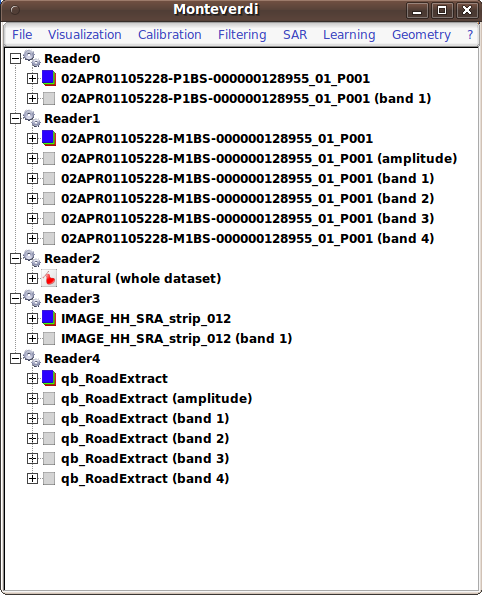
\includegraphics[width=0.44\textwidth]{monteverdi_mainwindow.eps}
   \itkcaption[Monteverdi main window]{Monteverdi main window.}
   \label{fig:mainwindow}
\end{figure}

This is Monteverdi's main window (figure \ref{mainwindow} )where the menus are available and where you can see the different 
modules which have been 
set up for the processing. Input data are obtained by readers. When you choose to use a new module, you select its input data,
 and therefore, you build a processing pipeline sequentially. 
Figure \ref{inputswindow} shows the generic window which allows to specify output(s) of Monteverdi's modules. 
 
\begin{figure}
   \center
   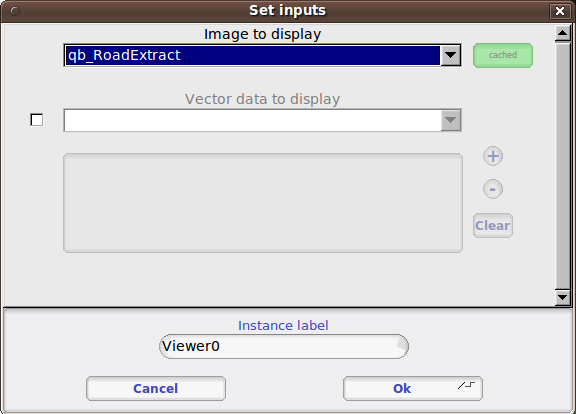
\includegraphics[width=0.44\textwidth]{monteverdi_inputs_window.eps}
   \itkcaption[Monteverdi main window]{Monteverdi inputs selection generic window.}
   \label{fig:inputswindow}
\end{figure}
Let's have a look at the different menus. The first one is of
 course the "File" menu. This menu allows you to open a data set, to save it and to cache it. The "data set" concept is
 interesting, since you don't need to define by hand if you are looking for an image or a vector file. Of course, 
you don't need to do anything special for any particular file format. So opening a data set will create a "reader" 
which will appear in the main window. At any time, you can use the "save data set" option in order to store to a 
file the result of any processing module.




\section{Open an image with Monteverdi}
The application allows to interactively select raster/vector dataset by browsing your PC. Monteverdi takes
advantage of the automatic detection of images' extensions to indicate the dataset type (optical, SAR or vector data).   

The input dataset is added to the "Data and Process" tree whcich describes the dataset content and each node corresponds to a layer.

\section{Visualize an image with Monteverdi}
This module allows to visualize raster or vector data. It allows to create RGB composition from the imput rasters. It is also possible to add 
vector dataset which are automatically reproject in the same projection of the input image or Digital Elevation informations. 

The viewer offers three types of data visualisation: 

\begin{itemize}
\item The scroll Window : to navigate quickly inside the entire scene
\item The Full resolution window: the view of the region of interest selected in the scroll window 
\item The Zoom window
\item The Pixel description: give access to dynamic informations on the current pixel pointed. Informations display are:
  \begin{itemize}
  \item The current index
  \item The pixel value 
  \item The computed value (the dynamic of hte input image is modify to get a proper visualisation
  \item The coordinates of the current pixel (long/lat)
  \item In case where there is a Internet connection available, Monteverdi displays the estimate location of the current pixel (country + city)  
  \end{itemize} 
\end{itemize}

\begin{figure}
   \center
   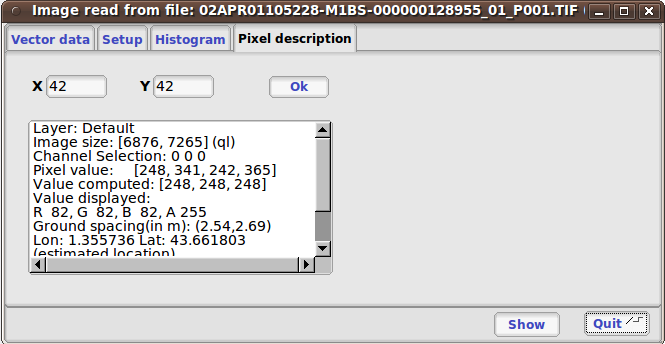
\includegraphics[width=0.44\textwidth]{monteverdi_viewer_pixel_description.eps}
   \itkcaption[Monteverdi main window]{Monteverdi pixel description box.}
   \label{fig:viewerpixeldescription}
\end{figure}

The Visualization offers others great functionnalities which are available in the detached window.
Figure \ref{viewervectordata} emphase the possibility It is possible to superpose vector dataset
to the raster image (see Figure \ref{viewervectordata}).

\begin{figure}
   \center
   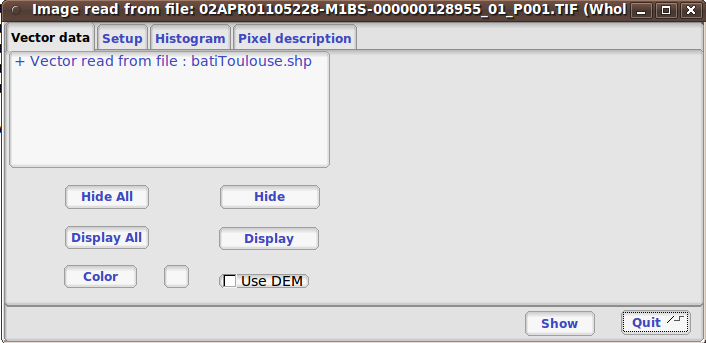
\includegraphics[width=0.44\textwidth]{monteverdi_viewer_vector_data.eps}
   \itkcaption[Vector Data visualization]{Monteverdi pixel description box.}
   \label{fig:viewervectordata}
\end{figure}

The "Setup Tab" allow to modify the RGB composition or use the grayscale mode to display only one layer. 

\begin{figure}
   \center
   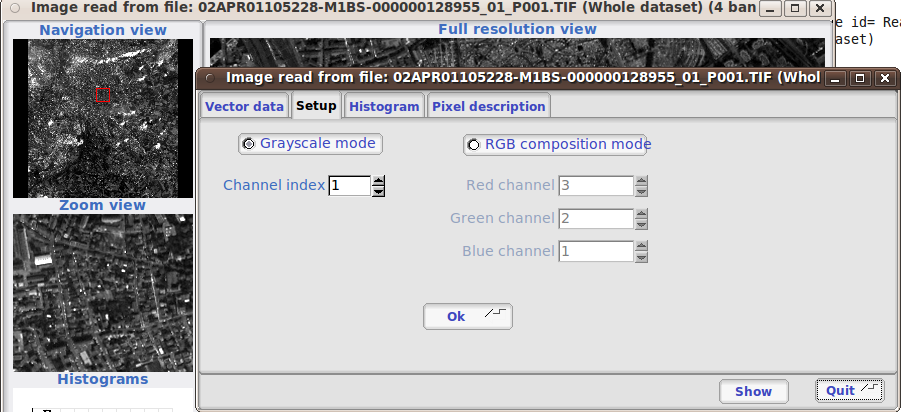
\includegraphics[width=0.44\textwidth]{monteverdi_viewer_rgb_composition.eps}
   \itkcaption[Manage RGB composition]{Manage RGB composition.}
   \label{fig:rgbcomposition}
\end{figure}

The "Histogram Tab" get access to the dynamic of the displayed layers. The basic idea is to Convert the output of the 
pixel representation to a RGB pixel on unsigned char to be displayed on screen. 
Values are contrained to 0-255 with a transfer function and a clamping operation.
By default, the dynamic of each layer is modified by
clamping the histogram at $min + 2\%$ and $max - 2\%$. 

\begin{figure}
   \center
   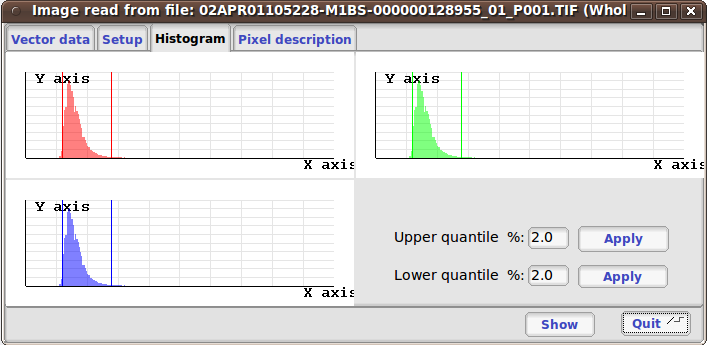
\includegraphics[width=0.44\textwidth]{monteverdi_viewer_histogram.eps}
   \itkcaption[Manage the dynamic of each layer]{Manage the dynamic.}
   \label{fig:histogram}
\end{figure}

There is also possible to select pixel coordinates and get access to all the informations abvailable in the Pixel description 
Box.

\begin{figure}
   \center
   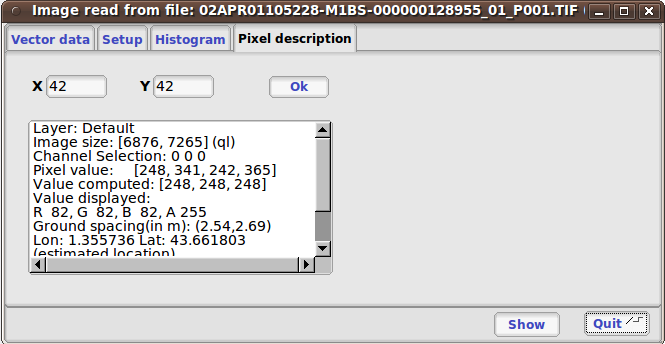
\includegraphics[width=0.44\textwidth]{monteverdi_viewer_pixel_description.eps}
   \itkcaption[Pixel description via index selection]{Index description via index selection.}
   \label{fig:pixeldescriptioninformations}
\end{figure}

\section{Cache dataset}
The "cache data set" (Figure \ref{cachingmodule}) is a very interesting thing. As you know, OTB implements processing on demand, so when you build a 
processing pipeline, no processing takes place unless you ask for it explicitly. That means that you can plug together
 the opening of a data set, an orthorectification and a spleckle filter, for example, but nothing will really be computed 
until you trigger the pipeline execution. This is very convenient, since you can quickly build a processing pipeline and 
let it execute afterwards while you have a coffee. In Monteverdi, you execute the processing by saving the result of the 
last module of a pipeline. However, sometimes, you may want to execute a part of the pipeline without wanting to give a 
name to the obtained result. You can do this by caching a data set. That is, the result will be stored in a temporary 
file which will be created in the "Caching" directory created by the application. Another situation in which you may need 
to cache a data set is when you need the input of a module to exist when you set its parameters. This is nor a real requirement, 
since Monteverdi will generate the needed data by streaming it, but this can be inefficient. This for instance about visualization
 of the result of a complex processing. Using streaming for brwsing through the result image means processing the visible part 
every time you move inside the image. Caching the data before visualization generated the whole data set in advance allowing 
for a more swift display. All modules allow you to cache their input data sets.

\begin{figure}
   \center
   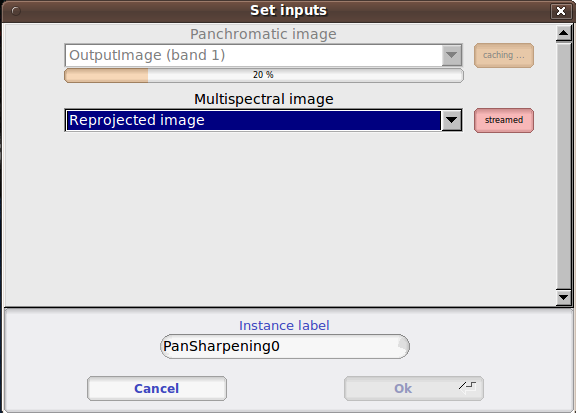
\includegraphics[width=0.44\textwidth]{monteverdi_caching_module.eps}
   \itkcaption[Cache operation on the panchromatic image in progress]{Cached and streamed dataset.}
   \label{fig:pixeldescriptioninformations}
\end{figure}

\chapter{Architecture of the application}
\section{Dynamic GUI definition}
The aim of Monteverdi is to provide a generic interface which is based on the definition of the internal processes. 
In this frame, the way that that you have to manage modules are identical during the definition of a new processes.
Selecting a module on the upper main window, open automatically the "Inputs definition Window" wich allow to select data which
are inputs of the current module. Monteverdi module can manage single or multiple inputs and these inputs can be images on your 
DD or results of previous module already registered in the "Data and Process" tree.    
\section{Dynamic I/O definition}
Management of image formats in Motneevrdi works in the manner as in the OTB library.
The principle is that the software automatically recognise the image format and.
The way that
Communication between modules follow also the same principle and the Input definition of modules request to all available
outputs of the same type in the "Data and process" tree.
Internally, all the treatments in Monteverdi are compute in Float precision by default. It is also possible to switch to Double 
precision by compiling the application from source and set the CMAKE option compile float to ON.
 

\section{Dynamic chain process}
fdsfsdfsdf

\chapter{Available modules}
\section{I/O operations}
\subsection{Extract region of interest}
It allows to extract regions of interest (ROI) from an image. There are two ways to select the region:
\begin{itemize}
\item By indicating the X and Y coordinatres of the upper-left coordinates and the X-Y size of the regions.
\item By interactivelly selecting the region of interest in the input image.
\end{itemize}

\subsection{Concatenate image bands}
With Monteverdi, you could generate a large scale of value added informations from lots of inputs data. One of the basic
functionnality is to be able to superpose result's layers into the same dataset.  
Concatenating images into one single multi-band image (they need to have the same size), and to be able to create RGB composition 
with the inputs layer.

\begin{figure}
   \center
   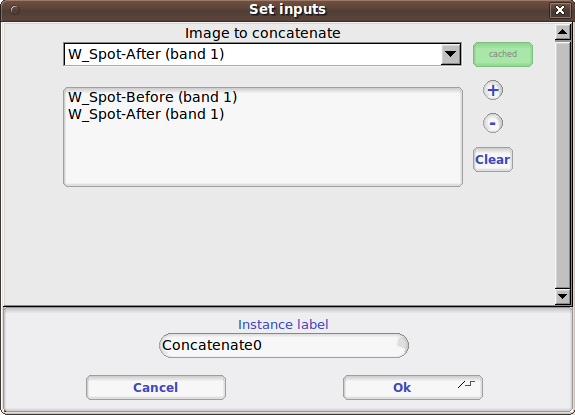
\includegraphics[width=0.44\textwidth]{monteverdi_concatenate_before_after.eps}
   \itkcaption[Concatenation of multitemporal data]{Concatenation module.}
   \label{fig:concatenate}
\end{figure}
 
\section{Geometric process}
In the frame of remote sensing process, the first operation is often to be able to superpose and maipulate imageries which 
come from different sources.
This section gives access to a large set of geometric operations.
It performs re-projection and orthorectification operations on Optical or SAR imageries using the available sensor models 
(image informations available in the meta-data are automatically read by the application).  
\subsection{Orthorectification}
The application is derived from the otbOrthorectificationApplication and allow to produce orthorectified imagery from level 1 
product.
The application is able to parse metadata informations and set default parameters. The application contains 4 tabs:

\begin{itemize}
\item Coordinates: Define the center or upper-left pixel coordinates of the orthorectified image (the Long/Lat coordinates are 
calculated through meta-data informations. It is also possible to specify the map projection of the output.
\item Output image: The module allow to only orthorectified a Region Of interest inside the input dataset. This tab allow the X and Y size 
around the center pixel coordinate or from the upper left index. The orthorectified imagery can also be resample at any resolution in the
line or column directions by setting the "Spacing X" and the "Spacing Y" and choosing the method of interpolation.
\item DEM: Indicate path to a directory containing SRTM elevation file. The application is able to detect inside the direcory which 
DEM files are relevant in the process.
\item Image extent: Compare the initial image extension with the preview the orthorectified result. This preview is automatically 
updated if the user change the "Size X" or "Size Y" values in the "Output Image" tab.   
\end{itemize}

\begin{figure}
   \center
   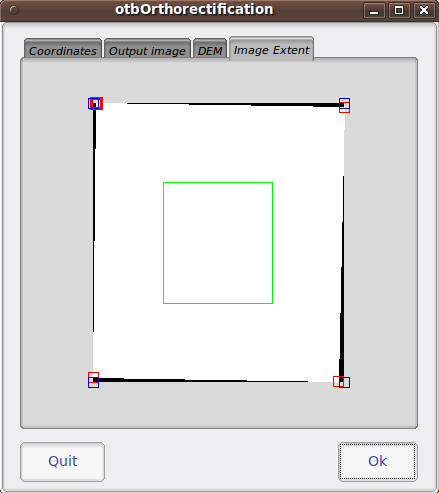
\includegraphics[width=0.44\textwidth]{monteverdi_ortho_extent.eps}
   \itkcaption[Preview of the orthorectified imagery]{Orthorectification module.}
   \label{fig:concatenate}
\end{figure}

\subsection{Re-projection module}
Allow raster reprojection of raster images.
\subsection{Registering 2 images by taking homologous point}
This module allows to register two images by taking separately homologous points in the reference image and in the image 
that you need to register. The principle is to estimate a transformation with the list of points.
The output of the module the input image that you need to register where the calculate transformation was applied. 

\begin{figure}
   \center
   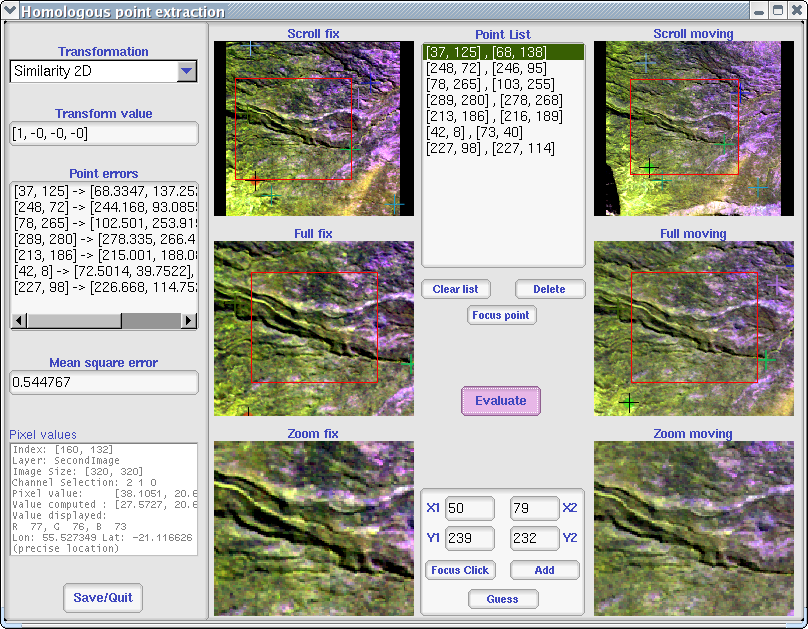
\includegraphics[width=0.44\textwidth]{monteverdi_homologous_point.eps}
   \itkcaption[Estimate transformation between 2 images]{Homologous point module.}
   \label{fig:concatenate}
\end{figure}


\subsection{Estimating sensor model based on ground control points}
This module allows to take ground copntrol points on a raster image where you 
This GCPs list is making correspondence between pixel coordinate in the input image and physical coordinates. The list
allows to derive a general function which to translate any pixel coordinates in physical positions. This function is 
based on a RPC transformation (Rational Polynomial Coefficients). As a consequence, the module enriches the output image 
with metadata informations defining a RPC sensor model associated with the input raster. 
There is several ways to generate the GCPs:

\begin{itemize}
\item With a Internet connection: Dynamically generate the correspondence on the input image and Open Street Map layers
\item Without an  Internet connection
\end{itemize}

It is also possible to import/export the GCP list from/to an XML file.

This output image could be without getting any geometric informations. Moreover, if the input image have already GCPs
in its metadata, the module allows to add or remove points from the existing list which is automatically loaded.       

\section{Calibration}
The basic idea is to be able to  
\subsection{Optical calibration}
In the case of the Optical calibration, the basic idea is to be able to retrieve reflectance of the observed physical object.
The input image contains only numerical which 
The process can be split in 3 main operations:
\begin{itemize}
\item Derived luminance from the numerical count in the input image. 
\item Convert the Luminance to Reflectance to produce the TOA(Top Of Atmosphere) image.
\item Inverse a radiative transfer code which simulate the reflection of solar radiation by a coupled atmosphere-surface system. This step produce 
the TOC (Top of Canopy) imagery which is the final result of the Optical calibration module. 
\end{itemize}
    
The module produce also a calculeted product which the TOC - TOA image.

\subsection{SAR calibration}

The calibration and validation of the measurement systems are important to maintain the
reliability and reproducibility of the SAR measurements but the establishment of correspondence between quantities measured 
by SAR and physical measure requires scientific background. The SAR calibration module allow to estimate quantitative accuracy
from Terra SAR X.
Describe the outputs!!!

\section{Filtering Operations}
\subsection{Band Math}
The Band Math module allow to perform simple mathematical operations (addition, substraction, multiplication) on 2 images. 
An operational example, on how this simple module can produce reliable information.
In rapid mapping context, it allows to compare easily . Figure XX shows the result of the substraction of water indices . The diiference was produce by the band math module
and allow to get a reliable estimation of the flood events.
\subsection{Feature extraction}
\subsection{Mean-shift segmentation}
\section{Learning}
\subsection{Supervised classification}
\subsection{Non-supervised classification}
The supervised classification  module is based on the Kmeans algorithm (link to the doc).
The GUI allows to modify parameters of the algorithm and produce
\section{Specific SAR functionnalities}
This section give access to specific treatments related to the 


\part{Developper's guide}\label{part:developperguide}
\chapter{Module architecture}
\chapter{Starter toolkit}

% \part{Appendix}\label{part:appendix}
% % \chapter{Frequently Asked Questions}
% % \label{sec:FrequentlyAskedQuestions}
% % \section{Introduction}
\subsection{What is OTB?}
OTB, the ORFEO Toolbox is a library of image processing algorithms developed by CNES in the
frame of the ORFEO Accompaniment Program.
OTB is based on the medical image processing library ITK, \url{http://www.itk.org}, and offers
particular functionalities for remote sensing image processing in
general and for high spatial resolution images in particular.

OTB provides:
\begin{itemize}
\item image access: optimized read/write access for most of remote sensing
image formats, meta-data access, simple visualization;
\item sensor geometry: sensor models, cartographic projections;
\item radiometry: atmospheric corrections, vegetation indices;
\item filtering: blurring, denoising, enhancement;
\item fusion: image pansharpening;
\item feature extraction: interest points, alignments, lines;
\item image segmentation: region growing, watershed, level sets;
\item classification: K-means, SVM, Markov random fields;
\item change detection.
\end{itemize}


Many of these functionalities are provided by ITK and have been tested
and documented for the use with remote sensing data.

\subsection{What is ORFEO?}
ORFEO stands for Optical and Radar Federated Earth Observation.  In
2001 a cooperation program was set between France and Italy to develop
ORFEO, an Earth observation dual system with metric resolution: Italy
is in charge of COSMO-Skymed the radar component development, and
France of PLEIADES the optic component.

The PLEIADES optic component is composed of two "small satellites"
(mass of one ton) offering a spatial resolution at nadir of 0.7 m and
a field of view of 20 km. Their great agility enables a daily access
all over the world, essentially for defense and civil security
applications, and a coverage capacity necessary for the cartography
kind of applications at scales better than those accessible to SPOT
family satellites. Moreover, PLEIADES will have stereoscopic
acquisition capacity to meet the fine cartography needs, notably in
urban regions, and to bring more information when used with aerial
photography.

The ORFEO "targeted" acquisition capacities made it a system
particularly adapted to defense or civil security missions, as well as
critical geophysical phenomena survey such as volcanic eruptions,
which require a priority use of the system resources.


With respect to the constraints of the franco-italian agreement,
cooperations have been set up for the PLEIADES optical component with
Sweden, Belgium, Spain and Austria.

\subsubsection{Where can I get more information about ORFEO?}
At the PLEIADES HR web site: \url{http://smsc.cnes.fr/PLEIADES/}.

\subsection{What is the ORFEO Accompaniment Program?}
Beside the Pleiades (PHR) and Cosmo-Skymed (CSK) systems developments forming ORFEO, the dual and bilateral system (France - Italy) for Earth Observation, the ORFEO Accompaniment Program was set up, to prepare, accompany and promote the use and the exploitation of the images derived from these sensors.

The creation of a preparatory program is needed because of :
\begin{itemize}
  \item  the new capabilities and performances of the ORFEO systems (optical and radar high resolution, access capability, data quality, possibility to acquire simultaneously in optic and radar),
  \item the implied need of new methodological developments : new processing methods, or adaptation of existing methods,
  \item the need to realize those new developments in very close cooperation with the final users, the integration of new products in their systems.
\end{itemize}


This program was initiated by CNES mid-2003 and will last until 2009.
It consists in two parts, between which it is necessary to keep a strong interaction:
\begin{itemize}
\item A Methodological part,
\item A Thematic part.
\end{itemize}


This Accompaniment Program uses simulated data (acquired during airborne campaigns) and satellite images quite similar to Pleiades (as QuickBird and Ikonos), used in a communal way on a set of special sites. The validation of specified products and services will be realized with those simulated data

Apart from the initial cooperation with Italy, the ORFEO Accompaniment
Program enlarged to Belgium, with integration of Belgian experts in
the different WG as well as a participation to the methodological
part.

\subsubsection{Where can I get more information about the ORFEO
  Accompaniment Program?}
Go to the following web site:
\url{http://smsc.cnes.fr/PLEIADES/A_prog_accomp.htm}.

\subsection{Who is responsible for the OTB development?}
The French Centre National d'\'Etudes Spatiales, CNES, initiated the ORFEO
Toolbox and is responsible for the specification of the library. CNES
funds the industrial development contracts and research contracts
needed for the evolution of OTB.

\section{Licence}
\subsection{Which is the OTB licence?}
OTB is distributed under a free software licence:\\
\url{http://www.cecill.info/licences/Licence_CeCILL_V2-en.html}.


\subsection{If I write an application using OTB am I forced to distribute that application?}
No. The license gives you the option to distribute your application if
you want to. You do not have to exercise this option in the license.

\subsection{If I wanted to distribute an application using OTB what license would I need to use?}
    The CeCILL licence.

\subsection{I am a commercial user. Is there any restriction on the
  use of OTB?}
OTB can be used internally ("in-house") without restriction, but only
redistributed in other software that is under the CeCILL licence.

\section{Getting OTB}

\subsection{Who can download the OTB?}
Anybody can download the OTB at no cost.

\subsection{Where can I download the OTB?}
Go to \url{http://www.orfeo-toolbox.org}
 and follow the "download OTB" link. You will have access to the OTB
source code and to the Software User's Guide.

\subsection{How to get the latest bleeding-edge version}\label{sec:FAQMercurial}

You can get the current version as our repository is public using mercurial (available at \url{http://www.selenic.com/mercurial}). Be aware that, even if the golden rule is {\em what is commited will compile}, this is not always the case.

The first time, you can get the source code using:
\begin{verbatim}
      hg clone http://hg.orfeo-toolbox.org/OTB
\end{verbatim}

Then you can build OTB as usual using this directory as the source (refer to build instruction).

Later if you want to update your source, from the OTB source directory, just do:
\begin{verbatim}
      hg pull -u
\end{verbatim}

A simple \texttt{make} in your OTB binary directory will be enough to update the library (recompiling only the necessary stuff).


\section{Installing OTB}
\label{sec:FAQInstall}
\subsection{Which platforms are supported}
OTB is a multi-platform library. It has successfully been installed on
the following platforms:
\begin{itemize}
  \item Linux/Unix with GCC (2.95.X, 3.3.X, 4.1.X, 4.2.X, 4.3.X).
  \item Windows with Microsoft Visual Studio C++ 7.1 .NET 2003.
  \item Windows with Microsoft Visual Studio C++ 8.0 .NET 2005.
  \item Windows with MinGW. (mingw + msys at \url{http://www.mingw.org})
  \item Cygwin. (\url{http://www.cygwin.com})
  \item MacOS
\end{itemize}

Support for the following platforms is planned:
\begin{itemize}
  \item Windows with Microsoft Visual Studio C++ 6.0.
\end{itemize}

\subsection{Which libraries/packages are needed before installing
 OTB?}
\begin{itemize}
\item CMake (\url{http://www.cmake.org})
\item GDAL (\url{http://www.gdal.org})
\item Optional (you may use the version included in OTB): Fltk (\url{http://www.fltk.org}) and ITK (\url{www.itk.org})
\item Optional (OTB will compile but some small functionalities will be missing): cURL (\url{http://curl.haxx.se/}), FFTW (\url{www.fftw.org}).
\end{itemize}

\subsection{Main steps}
In order to install OTB on your system follow these steps (in the
given order):
\begin{enumerate}
  \item Install CMake (binary packages are available for most platforms).
  \item Install GDAL (binary packages are available for most platforms).
%   \item Install Fltk using the CMake scripts. Do not use the
%   \texttt{configure} approach or the project files for Microsoft
%   Visual Studio shipped with Fltk.
%   \item Install ITK if you do not want to use the ITK version provided
%   with OTB. Use CMake for the configuration.
  \item Install OTB using CMake for the configuration.
\end{enumerate}

We assume that you will install everything on a directory called
\texttt{INSTALL\_DIR}, which usually is \texttt{/usr/local}, \texttt{/home/jordi/local} or
whatever you want. Make sure that you have downloaded the source code for:
  \begin{itemize}
  \item CMake (\url{http://www.cmake.org})
  \item GDAL (\url{http://www.gdal.org})
%   \item Fltk (\url{http://www.fltk.org})
  \end{itemize}

\subsubsection{Unix/Linux Platforms}

\textbf{Important note}: on some Linux distributions (eg. Debian, Ubuntu, Fedora), you should use
the official packages for CMake, GDAL and Fltk. Once you have installed these
packages, you can skip to step 4.

\begin{enumerate}

\item Install GDAL (or \textbf{use your distribution package})
  \begin{verbatim}
      cd INSTALL_DIR
      gunzip gdal.1.5.2.tar.gz
      tar xvf gdal.1.5.2.tar
      cd gdal.1.5.2
      ./configure --prefix=INSTALL_DIR
      make
      make install
  \end{verbatim}

It seems to be a bug in the GDAL install procedure: if you are installing it without root privileges, even if your \texttt{INSTALL\_DIR} is a directory for which you have the write permissions, GDAL tries to copy the python bindings together with the Python site packages, which are usually somewhere in /usr/lib.

Actually, since this is the last step in the GDAL install procedure, when you get the error message, the GDAL libs and header files are already installed, so you can safely ignore the error.

The \texttt{--without-python} option passed to the \texttt{configure} step avoids this. However, some users may want to have Python bindings, so recommending this option for the install may not be OK for everybody.

\item Install CMake (or \textbf{use your distribution package})
  \begin{verbatim}
      cd INSTALL_DIR
      gunzip cmake-2.6.0.tar.gz
      tar xvf cmake-2.6.0.tar
      cd cmake-2.6.0
      ./configure --prefix=INSTALL_DIR
      make
      make install
  \end{verbatim}
      In order to properly use cmake, add \texttt{INSTALL\_DIR/bin} to
      your path with \texttt{export PATH=\$PATH:INSTALL\_DIR/bin} or
      something similar.

\item Install Fltk (optional) using CMake (do not use the configure script) (or \textbf{use your distribution package})
  \begin{verbatim}
      cd INSTALL_DIR
      bunzip2 fltk-1.1.9-source.tar.bz2 OR
      gunzip fltk-1.1.9-source.tar.gz
      tar xvf fltk-1.1.9-source.tar
      mkdir Fltk-binary
      cd Fltk-binary
      ccmake ../fltk-1.1.9
      --> follow the CMake instructions, in particular:
          --> set CMAKE_INSTALL_PREFIX to INSTALL_DIR within CMake
	  --> set BUILD_EXAMPLES to ON within CMake
	  --> generate the configuration with 'g'
      make
      make install
      --> check that the examples located in
      INSTALL_DIR/Fltk-binary/bin work, in particular, the fractals
      example which makes use of the OpenGL library needed by OTB.
  \end{verbatim}

   You can also choose to use the FLTK version we included in the source of OTB, in this case, everything will be compile at the same time. To do that, you will have to set the option \texttt{OTB\_USE\_EXTERNAL\_FLTK} to \texttt{OFF}

\item Install OTB
  \begin{verbatim}
      cd INSTALL_DIR
      gunzip OrfeoToolbox-2.8.0.tgz
      tar xvf OrfeoToolbox-2.8.0.tar
      mkdir OTB-Binary
      cd OTB-Binary
      ccmake ../OrfeoToolbox-2.8.0
      --> follow the CMake instructions, in particular:
	  --> set BUILD_EXAMPLES to ON within CMake
	  --> set BUILD_SHARED_LIBS to ON within CMake
	  --> set BUILD_TESTING to OFF within CMake
	  --> set CMAKE_INSTALL_PREFIX to INSTALL_DIR within CMake
	  --> set GDAL_INCLUDE_DIRS to INSTALL_DIR/include within CMake
	  --> set GDAL_LIBRARY_DIRS to INSTALL_DIR/lib within CMake
	  --> set OTB_USE_EXTERNAL_ITK to OFF within CMake
	  --> set FLTK_DIR to INSTALL_DIR/Fltk-Binary within CMake OR
	      if you do not have FLTK press 't' to change to advanced
              mode and set OTB_USE_VISU to OFF
	  --> generate the configuration with 'g'
       make -j 2
  \end{verbatim}

  If you want a faster compilation and don't want the compilation of the examples, you
  can set \texttt{BUILD\_EXAMPLES} to \texttt{OFF}. Some plateforms apparently
  have more difficulties with shared libraries, if you experience any problem
  with that, you can set \texttt{BUILD\_SHARED\_LIBS} to \texttt{OFF} but the
  built size might reach 1~GB.

  After these steps, you have the source of OTB in \texttt{INSTALL\_DIR/OrfeoToolbox-2.8.0}
  and the compiled binaries and libraries in \texttt{INSTALL\_DIR/OTB-Binary}. Keeping
  the sources is important as most programs you will designed will need an access
  to the txx files during compilation. However, the binaries directory knows were
  its sources are and you will need to point only to the \texttt{INSTALL\_DIR/OTB-Binary}
  when the \texttt{cmake} for your program will ask you where the OTB is.

  If you want to put OTB in a standard location, you can proceed with:

  \begin{verbatim}
      make install
  \end{verbatim}

  but \textbf{this is only optional}.


\end{enumerate}

\subsubsection{Microsoft Visual Studio C++ 7.1}
\begin{enumerate}
\item Install GDAL

	Get the binary package from \url{http://www.gdal.org/} and follow the instruction to install. If it fail, proceed to the installation from the source.


        From source:

	MSVC++ 7.1 project files are needed to compile GDAL.

	These files can be downloaded at \url{http://vterrain.org/dist/gdal151-vc71.zip}.

	Then, unzip it to your GDAL folder, and it will create a folder (named "VisualStudio").

	Load the solution (.sln file) and build the gdal project.

	More details can be found at \url{http://vterrain.org/Distrib/gdal.html}.

% \item Install Fltk
%
% 	Use CMake on Windows to generate MSVC++ 7.1 project files from fltk sources.
%
% 	Open the solution and build the fltk project.

\item Install OTB

	Use CMake on Windows to generate MSVC++ 7.1 project files from otb sources.

	Set the \texttt{OTB\_USE\_EXTERNAL\_FLTK} option to \texttt{OFF}

	Open the solution and build the otb project.

\end{enumerate}

\subsubsection{Microsoft Visual Studio C++ 8.0}
\begin{enumerate}
\item Install GDAL (from source)

	Get the binary package from \url{http://www.gdal.org/} and follow the instruction to install. If it fail, proceed to the installation from the source.



        From source:

        Open a MS-DOS prompt.

        Run the VCVARS32.bat script that comes with the compiler (it can be found in
        Microsoft Visual Studio 8/VC/bin).

        Then, go to the GDAL root directory, and tape :
        \begin{verbatim}
                nmake /f makefile.vc
        \end{verbatim}

        Once the build is successful, tape this line to install GDAL :
        \begin{verbatim}
                nmake /f makefile.vc install
        \end{verbatim}

        More details about this install can be found at \url{http://www.gdal.org/gdal_building.html}.


% \item Install Fltk
%
% 	Use CMake on Windows to generate MSVC++ 8.0 project files from fltk sources.
%
% 	Open the solution and build the fltk project.

\item Install OTB

	Use CMake on Windows to generate MSVC++ 8.0 project files from otb sources.

	Set the \texttt{OTB\_USE\_EXTERNAL\_FLTK} option to \texttt{OFF}

	Open the solution and build the otb project.

\end{enumerate}

\subsubsection{MinGW on Windows platform}
\begin{enumerate}

\item Download the lastest version of mingw and msys at \url{http://www.mingw.org} and install those
	two programs.

	Then, launch MinGW : a prompt appears (similar to Linux one).

\item Install GDAL

	To compile GDAL, at configure step, use these options :
\begin{verbatim}
	./configure -prefix=INSTALL_DIR --host=mingw32 --without-libtool
	--without-python --with-png=internal --with-libtiff=internal
	--with-jpeg=internal
\end{verbatim}
	Then the usual make and make install.

% \item Install Fltk
%
% 	Generate MSYS Makefiles with CMake (Windows version) from fltk sources.
%
% 	Then, under prompt, tape make and make install where you have generated Makefiles with CMake.

\item Install OTB

	Similar to fltk install.

\end{enumerate}

\subsubsection{Cygwin}
\begin{enumerate}

\item Download the lastest version at \url{http://www.cygwin.com} and install it.
	Then, launch it, a prompt appears (similar to Linux one).

\item Install GDAL

	To compile GDAL, at configure step, use these options :
\begin{verbatim}
	./configure --prefix=INSTALL_DIR --with-png=internal --with-libtiff=internal
	--with-jpeg=internal
\end{verbatim}
	Then the usual make and make install.

% \item Install Fltk
%
% 	See Linux part for details (same procedure).

\item Install OTB

	See Linux part for details (same procedure).
\end{enumerate}

That should be all! Otherwise, subscribe to
   otb-users@googlegroups.com and you will get some help.

\subsection{Specific platform issues}
\subsubsection{SunOS/HP UX}
Due to a bug in the tar command shipped with some versions of SunOS,
problems may appear when configuring, compiling or installing OTB.

See \url{http://www.gnu.org/software/tar/manual/tar.html#Checksumming} for
details on the bug characterization.

The solution is to use the GNU tar command if it is available on your
system (gtar).

\subsubsection{Linux Debian/Ubuntu}
If you used the official gdal package version 1.4.0, the library is named
\texttt{libgdal1.4.0.so} so you have to create a simlink named
\texttt{libgdal.so}: \texttt{ln -s /usr/lib/libgdal1.4.0.so /usr/lib/libgdal.so}.

\subsubsection{Cygwin}
Due to an unknown bug, Fltk can't compile on some versions of Cygwin (OpenGL problems).

Put OTB\_USE\_VISU to OFF to avoid these problems.

Some bugs can appear while compiling GDAL with JPEG2000 files : disable this format to solve the problem.

\subsubsection{MSVC++ 8.0}
Execution errors can appear on some platforms, using GDAL compiled with MSVC++ 8.0.

This problem can be solved by downloading GDAL binaries for Windows
at \url{http://vterrain.org/Distrib/gdal.html}.

\section{Using OTB}

\subsection{Where to start ?}

OTB presents a large set of features and it is not always easy to start using it.
After the installation, you can proceed to the tutorials (in the Software Guide).
This should give you a quick overview of the possibilities of OTB and will teach
you how to build your own programs.

\subsection{What is the image size limitation of OTB ?}

The maximum physical space a user can allocate depends on her platform. Therefore,
image allocation in OTB is restricted by image dimension, size, pixel type and number
of bands.

Fortunately, thanks to the streaming mechanism implemented within
OTB's pipeline (actually ITK's), this limitation can be bypassed. The
use of the \doxygen{otb}{StreamingImageFileWriter} at the end of the pipeline,
or the \doxygen{itk}{StreamingImageFilter} at any point of the pipeline will
seamlessly break the large, problematic data into small pieces whose
allocation is possible. These pieces are processed one afther the
other, so that there is not allocation problem anymore. We are often working with
images of $25000 \times 25000$ pixels.

For the streaming to work, all the filters in the pipeline must be streaming capable
(this is the case for most of the filters in OTB). The output image format also need to be
streamable (not PNG or JPEG, but TIFF or ENVI, for instance).

To tune the size of the streaming pieces, the OTB has
two CMake variables. The first is named
OTB\_STREAM\_IMAGE\_SIZE\_TO\_ACTIVATE\_STREAMING. It represents the
minimum size of the image in bytes for which streaming may be helpful. The
second, OTB\_STREAM\_MAX\_SIZE\_BUFFER\_FOR\_STREAMING, specifies the
maximum size in bytes a streaming piece should have. It can be used to
compute the optimal number of pieces to break the input data into.

These two parameters have been used in the OTB-Applications/Utils/
applications. Take this as an example of how they can be used. They
can also be tuned by the user to match her specific needs.


\section{Getting help}
\subsection{Is there any mailing list?}
Yes. There is a discussion group at
\url{http://groups.google.com/group/otb-users/} where you can get help
on the set up and the use of OTB.

\subsection{Which is the main source of documentation?}
The main source of documentation is the OTB Software Guide which can
be downloaded at
\url{http://www.orfeo-toolbox.org/packages/OTBSoftwareGuide.pdf}. It
contains tenths of commented examples and a tutorial which should be a good starting
point for any new OTB user. The code source for these examples is
distributed with the toolbox. Another information source is the
on-line API documentation which is available at \url{http://orfeo-toolbox.sourceforge.net/Doxygen}.

\section{Contributing to OTB}\label{sec:contributing}

\subsection{I want to contribute to OTB, where to begin?}

First, you can send an email to otb@cnes.fr to let us know what functionality
you would like to introduce in OTB. If the functionality seems important for the
OTB users, we will then discuss on how to send your code,
make the necessary adaptions, check with you that the results are correct and finally
include it in the next release.

You can also run the nightly tests so we have a wider range of plateforms to detect the
bug faster. Look at section \ref{sec:runningTheTests}.

\subsection{What are the benefits of contributing to OTB?}

Besides the satisfaction of contributing to an open source project, we will include
the references to relevant papers in the software guide. Having algorithms
published in the form of reproducible research helps science move faster and
encourages people who needs your algorithms to use them.

You will also benefit from the strengths of OTB: multiplatform, streaming and
threading, etc.

\subsection{What functionality can I contribute?}

All functionalities which are useful for remote sensing data are of interest. As
OTB is a library, it should be generic algorithms: change, detection, fusion,
object detection, segmentation, interpolation, etc.

More specific applications can be contributed to the OTB-Applications package.

\section{Running the tests}\label{sec:runningTheTests}

\subsection{What are the tests?}

OTB is an ever changing library, it is quite active and have scores of changes per day from different people. It would be a headache to make sure that the brand new improvement that you introduced didn't break anything without automated tests. You also have to take into account the different OS, compilers, options, versions of external libraries, etc.

For each class, at minimum there is a test which tries to instantiate it and another one which uses the class. The output of each test (image, text file, binary file) is controlled against a baseline to make sure that the result hasn't change.

All these test are available in the directory \texttt{Testing} and are also good examples on how to use the library.

\subsection{How to run the tests?}

There is more than 1000 tests for OTB and about 100 for the applications and it takes from 20 minutes to 3 hours to run all the test, mainly depending on your compilation option (Release mode does make a difference) and of course your hardware.

To run the test, you first have to make sure that you set the option \texttt{BUILD\_TESTING} to \texttt{ON} before building the library. If you want to modify it, just rerun ccmake, change the option, then make.

For some of the test, you also need the test data and the baselines (see below).

Once OTB is built with the test, you just have to go to the binary directory where you built OTB and run \texttt{ctest -N} to have a list of all the tests. Just using \texttt{ctest} will run all the tests. To select a subset, you can do \testtt{ctest -R Kml} to run all tests related to kml files or \texttt{ctest -I 1,10} to run tests from 1 to 10.

\subsection{How to get the test data?}

Tests data are also controlled by mercurial (see \ref{sec:FAQMercurial}).

You can get the base doing:
\begin{verbatim}
      hg clone http://hg.orfeo-toolbox.org/OTB-Data
\end{verbatim}

This is about 1~GB of data, so it will take a while, but you have to do it only once, as after, a simple
\begin{verbatim}
      hg pull -u
\end{verbatim}
will update you to the latest version of the repository.


\subsection{How to submit the results?}

Once you know how to run the test, you can also help us to detect the bugs or configuration problems specific to your configuration. As mentionned before, the possible combination between OS, compiler, option, external libraries version is too big to be tested completely, but the more the better.

You just have to launch ctest with the \texttt{-D Experimental} switch. Hence:
\begin{verbatim}
      ctest -D Experimental
\end{verbatim}

If you are interested in setting up a nightly test (automatically launched every night), please contact us and we will give you the details.

\section{OTB's Roadmap}

\subsection{Which will be the next version of OTB?}
OTB's version numbers have 3 digits. The first one is for major
versions, the second one is for minor versions and the last one is for
bugfixes.

The first version was 1.0.0 in July 2006. Version 1.2.0, 1.4.0 and 1.6.0 were
released in between. The 2.0.0 major version  was released in December 2007.
The 2.2.0, 2.4.0 and 2.6.0 in June, July and November 2008 respectively.
The current one is 2.8.0.

\subsubsection{What is a major version?}
A major version of the library implies the addition of high-level
functionalities as for instance image registration, object recognition, etc.

\subsubsection{What is a minor version?}
A minor version is released when low-level functionalities are
available within one major functionality, as for instance a new
change detector, a new feature extractor, etc.

\subsubsection{What is a bugfix version?}
A bugfix version is released when significant bugs are identified and fixed.

\subsection{When will the next version of OTB be available?}
We plan to release major new OTB version once a year, that is, version
2.0.0 was available at the end of 2007, version 3.0.0 should be released
by the beginning of 2009, and so on.

\subsection{What features will the OTB include and when?}
There is no detailed plan about the availability of OTB new features,
since OTB's content depends on ongoing research work and on feedback
from thematic users of the ORFEO Accompaniment Program.

Nevertheless, the main milestones for the OTB development are the
following:
\begin{itemize}
  \item{Version 1 (2006):}
    \begin{itemize}
    \item core of the system,
    \item IO,
    \item basic filtering, segmentation and classification,
    \item basic feature extraction,
    \item basic change detection.
    \end{itemize}
    \item{Version 2 (2007):}
      \begin{itemize}
      \item geometric corrections,
      \item radiometric corrections,
      \item registration.
      \end{itemize}
    \item{Version 3 (2008):}
      \begin{itemize}
      \item multi-scale and multi-resolution analysis,
      \item object detection and recognition,
      \item supervised learning.
      \end{itemize}
    \item{Version 4 (2009):}
      \begin{itemize}
	\item data fusion,
	\item spatial reasoning.
      \end{itemize}

\end{itemize}

%% \subsection{When will feature X or Y be included in OTB?}

% 
% \chapter{Release Notes}
% \label{sec:ReleaseNotes}
% \verbatiminput{RELEASE_NOTES.txt}


%Comment generation of wrapping documentation for release 3.2
% \chapter{Wrappings to other languages}
%Set the code style to Java for the Wrapping

% \section{OTB-Wrapping: bindings to Java language}
OTB-Wrapping is a project designed to allow classes from OTB 
to be wrapped for use with languages like Python, and Java and Tcl. 
The project is based on CMake. SWIG, CableSwig and finally OTB that must be already built.
 The OTB-wrapping project is an extension of the project WrapITK \url{http://code.google.com/p/wrapitk/}. 
It allows the Python, Java and Tcl users to have program written in their own language to use the classes and 
the capabilities of OTB.
Since OTB-Wrapping provides an interface to some C++ compiled code, execution times are very similar to C++ 
pure programs in most cases.
Once the project compiled, one can use the wrapped classes to write programs in your favorite language.
The OTB Tutorials were translated in Java and can use the OTB capabilities to show how to use the 
Orfeo Toolbox easily. 

\subsection{Mangling}
You probably noticed that class names are quite barbaric. It is due to the
mangling. With the Java versions less or equal to 1.6, no generic programming is
allowed. It means that no templates can be used. Then, to use a C++  class in Java, the class generated 
(called proxies) are templated with the available types and for each type a Java
proxy is generated. The mangled types are concatenated and added in the end of
the class. For instance, when one want to use the \doxygen{otb}{Image} with the pixel type float 
and the dimension 2, the class generated will be otbImageF2.

The table ~\ref{tab:basictypetomangle} summarize the mangling used for the basic types. 

\begin{table}[!htbp]
\begin{center}
\begin{tabular}{|c|c|}
\hline
Type                  &  Mangle used  \\
\hline
float                 &  F         \\
double                &  D         \\
unsigned char         &  UC        \\
unsigned short        &  US        \\
unsigned long         &  UL        \\
bool                  &  B         \\

\hline 
\end{tabular}
\caption{Mangling of the basic types used.}\label{tab:basictypetomangle}
\end{center}
\end{table}

In OTB, there are some types used in several classes like \doxygen{otb}{Image} and  \doxygen{otb}{VectorImage}, or \doxygen{otb}{VectorData}.
Then those classes have their own mangling two. The table ~\ref{tab:typetomangle} shows some of the mangled classes. 

\begin{table}[!htbp]
\begin{center}
\begin{tabular}{|c|c|}
\hline
OTB Type                  &  Mangle used  \\
\hline
otb::Image                 &  I         \\
otb::VectorImage           &  VI        \\
otb::VectorData            &  VD        \\
\hline 
\end{tabular}
\caption{Mangling of the usually types used.}\label{tab:typetomangle}
\end{center}
\end{table}


The mangled name otbImageF2 means that we are dealing with the class otb::Image with 
template arguments float and 2. So, otbImageF2 is equivalent to \verb|otb::Image<float,2>|. Another example 
can be otbImageFileReaderIF2, knowing that I (~\ref{tab:typetomangle}) is the mangle for otb::Image, F is the mangle 
for the type float then IF2 is the mangle for \verb|otb::Image<float,2>|, and
finally otbImageFileReaderIF2 is the mangle for \verb|otb::ImageFileReader< otb::Image< float,2 > >|.


\subsection{How to Use OTB-Wrapping in Java}

\subsubsection{Import OTB classes}
The OTB-Wrapping project provides some \verb|jar| files that corresponds to the
modules implemented in the directory Libraries. Each OTB-wrapping module is automatically wrapped to a separate Java package.
For instance, the directory Libraries contains the modules otbImages and
otbLearning. The jars produced will be \verb|org.otb.otbimages| and
\verb|org.otb.otblearning|. Those jars can be used as usual in Java.

To write an example that uses OTB classes, you have to import those jars in your program by adding the directive 
\verb?import org.otb.otbio.*?. You can then access to all the classes in the otbIO module (cf section \ref{sec:tuto}).

\subsubsection{Compile Java programs}
The next step is to compile the Java program. Note that the Java compiler needs some options like 
\begin{itemize}
\item The class path  : specifies where to find user class files. \\
      The option is  -classpath .:path\_to\_the\_jar1:path\_to\_the\_jar2.
\end{itemize}

\subsubsection{Java programs execution}
Now we can execute the Java class compiled, it needs some options too.
\begin{itemize}
\item The class path  : specifies where to find user class files.\\
      The option is -classpath .:path\_to\_the\_jar1:path\_to\_the\_jar2...
\item The java.library.path : A system property that specifies where the libraries are.\\
      The libraries are named moduleJava.\{ dll|so|dylib \}.
\end{itemize}

\begin{landscape}
\subsection{Example}

Here is a simple example written in C++, and its translation in Java. 


\begin{table}[!htbp]
\begin{center}
\begin{tabular}{|p{8.35cm}|p{9.75cm}|}
\hline
Example in C++                  &  Example translated in Java  \\
\hline

\verb$#include "otbImage.h"$                &       \verb$import org.otb.otbimage.*;$                                 \\
\verb$#include "otbImageFileReader.h"$      &       \verb$import org.otb.otbio.*;$                                    \\
\verb$#include "otbImageFileWriter.h"$      &                                                                        \\
                                            &                                                                         \\
\verb$void otbReaderWriter(Int argc,char * argv[]){$ & \verb$public class otbReaderWriter{$        \\
                                                     &  \verb$public static void main(String argv[]){$  \\
      
 //typedefs :                              &     //The typedefs step are not necessary since no generic \\
                                           &     //programmation is allowed in Java.    \\

\verb$typedef otb::Image<float,2>  ImageT;$             &           \\
\verb$typedef otb::ImageFileReader<ImageT> ReaderType;$  &           \\
\verb$typedef otb::ImageFileWriter<ImageT> WriterType;$  &            \\

                       &                                           \\
// Instanciation :     &                      // Instanciation :   \\

\verb$ReaderType::Pointer reader = ReaderType::New();$    & \verb$otbImageReaderIF2 reader = new otbImageReaderIF2();$ \\ 
\verb$WriterType::Pointer writer = WriterType::New();$    & \verb$otbImageFileWriterIF2 writer=new otbImageFileWriterIF2();$  \\

 & \\
 // Set the filenames                           & // Set the filenames \\
\verb$reader->SetFileName(argv[1]);$            & \verb$reader.SetFileName(argv[0]);$ \\
\verb$writer->SetFileName(argv[2]);$            & \verb$writer.SetFileName(argv[1]);$  \\
&\\
 // Plug the pipeline                           & // Plug the pipeline  \\
 
\verb$writer->SetInput(reader->GetOutput());$   &  \verb$writer.SetInput(reader.GetOutput());$    \\ 
 &\\
 // Trigger the pipeline execution              &  // Trigger the pipeline  execution\\
\verb$writer->Update();$                        &  \verb$writer.Update();$  \\
 
\hline 
\end{tabular}
\caption{C++ code translation.}\label{tab:translatedexample}
\end{center}
\end{table}


\end{landscape}

\subsection{Use OTB-Wrapping}

\subsubsection{Download sources}
The source code for the project OTB-Wrapping is available here: \\
\url{http://hg.orfeo-toolbox.org/OTB-Wrapping}

\subsubsection{Required Tools}
OTB-Wrapping required the release 3.2 of the Orfeo Toolbox or greater. This project required some tools and 
and libraries : 
\begin{itemize}
\item CMake (\verb!>2.6!) to configure the compilation system.
\item CableSwig (\verb!>0.1.0!) for parsing and automatic instanciation of C++ templates.\\
      The source code is available here: \url{http://www.itk.org/ITK/resources/CableSwig.html}
\item SWIG  (\verb!>1.3.40!) for language binding
\item Target Language development libraries (JRE for Java, Python 2.6 for Python).
\end{itemize}

\subsubsection{Compile OTB-Wrapping sources}
First, this project needs OTB, CableSwig and SWIG to be built. Once this step done, create a 
directory where the project will be compiled (don't compile in the sources directory).
The compilation can be done successfully following those steps :

\begin{itemize}
\item Run CMake (ccmake under Linux and MacOSX or cmake.exe under Windows) and specify the path to the sources.
\item Edit the paths for OTB, CableSwig and SWIG binary directories.
\item Turn the option \verb|WRAP\_ITK\_|(\verb|JAVA| | \verb|PYTHON| | \verb|Tcl|  )  to ON to choose your target language.
\item Choose the modules you want to wrap.
\item Configure the project and generate the solution.
\item Compile using make in the binary directory (on Linux and MacOSX), or open the solution (.sln)\\
      and generate the solution on Windows.
\end{itemize}

Once the compilation completed successfully, the directory \verb|lib| will contain several jars which are Java archives 
and the libraries corresponding to the modules. Those are the useful to use OTB capabilities in Java language.

\subsubsection{Download binaries}

Ready-to-use binaries are available for OTB-Wrapping project. You can find more informations in section~\ref{sec:install_binaries}. 

\subsubsection{Use OTB-Wrapping with Eclipse}
OTB-Wrapping produces Java archives and libraries that can be used with Eclipse. You can then create your Java 
project and use the OTB wrapped classes. 
Eclipse gives the possibility to add external jars. 
After creating a new project, 
\begin{itemize}
\item Run the project configuration (Run then Run Configurations) to add the externals OTB-Wrapping Jars.
      In the Classpath section, add external jars by searching the jars produced. (They are generally in directory lib).
\item Add the path to the OTB-Wrapping libraries to  the environment variable PATH. Go to the tab Environment 
      (always in Run Configurations setup), \emph{Select} the environment variable PATH, and add the complete path 
      to the location of the libraries.
\end{itemize}

You can now import the OTB wrapped classes in your own Java classes, like shown in section \ref{sec:tuto}.


\normalsize

\section{Java tutorials}\label{sec:tuto}
\lstsetjava
\subsection{Hello World}
\input{HelloWorldOTBJava.tex}

\subsection{Pipeline}
\input{PipelineJava.tex}

\subsection{Filtering pipeline}
\input{FilteringPipelineJava.tex}

\subsection{Smarter Filtering Pipeline}
\input{SmarterFilteringPipelineJava.tex}

\subsection{Scaling Pipeline}
\input{ScalingPipelineJava.tex}

\subsection{MultiSpectral}
\input{MultiSpectralJava.tex}

\subsection{OrthoFusion}
\input{OrthoFusionJava.tex}


\normalsize
\section{Python tutorials}\label{sec:tutoPython}
\lstsetpython
\subsection{Hello World}
\input{HelloWorldPython.tex}

\subsection{Pipeline}
\input{PipelinePython.tex}

\subsection{Filtering pipeline}
\input{FilteringPipelinePython.tex}

\subsection{Smarter Filtering Pipeline}
\input{SmarterFilteringPipelinePython.tex}

\subsection{Scaling Pipeline}
\input{ScalingPipelinePython.tex}

\subsection{MultiSpectral}
\input{MultiSpectralPython.tex}

% \subsection{OrthoFusion}
% \input{OrthoFusionPython.tex}



\section{Developer Guide}\label{sec:dev}

\subsection{Add a new Library : Creating a new CMakeList.txt file}
Each OTB-Wrapping sub-library (e.g. itkBase, or otbChangeDetection) 
lives in a sub-directory of the OTB-Wrapping project (within the Libraries directory)
 with a CMakeLists.txt file that describes how that library and its language support files 
(e.g. Java template definitions) is to be created. 
See SampleCMakeLists.txt in the Documentation directory for a description of each macro and option that
can appear in such a file. What follows is the usual set of commands that will appear:

\small
\verb$WRAP_LIBRARY("otbMySpatialObjectExtensions")$ \\
\verb$SET(WRAPPER_LIBRARY_DEPENDS itkSpatialObject itkBase)$ \\
\verb$SET(WRAPPER_LIBRARY_LINK_LIBRARIES ITKCommon )$ \\
\verb$AUTO_INCLUDE_MODULES()$ \\
\verb$END_WRAP_LIBRARY()$ \\
\normalsize

\begin{itemize}
\item \verb$WRAP_LIBRARY$  sets up the environment to wrap a set of classes into a 
      library with a given name. This macro is defined in TypedefMacros.cmake. 
\item \verb$WRAPPER_LIBRARY_DEPENDS$ stores the list of OTB-Wrapping libraries on which the current library\\
      depends (e.g. which libraries like otbImages or otbChangeDetection, are going to be used in the \\
      current library). 
\item \verb$WRAPPER_LIBRARY_LINK_LIBRARIES$ stores a set of other libraries to add at link time. 
These can be 3rd party libraries that you will use 
(be sure to properly set \verb$LINK_DIRECTORIES$ in this case), 
or more commonly, the OTB libraries that need to 
be linked in, like OTBCommon, OTBIO, etc.
\item \verb$AUTO_INCLUDE_MODULES()$  edits the list of the headers that have to 
      be included by scanning all the cmake files present in the modules. This macro is implemented in the 
      file TypedefMacros.cmake.

\item \verb$END_WRAP_LIBRARY()$ is needed to check several things. First, it checks if all the dependecies 
      of the current library are wrapped. Secondly, it calls the right macro relative to the language selected
      in order to creates rules to parse the CableSwig inputs and compile a wrapper library. 
\end{itemize}

\subsection{Add a new cmake file}
A \verb$wrap_XXX.cmake$ file defines a group of classes and/or template instantiations to be wrapped. 
Most of the time, one such file is defined for each class wrapped, but this is not strictly necessary. 
Within such a file, directives are issued to wrap classes and particular template instances.
OTB-Wrapping define several macros and variables designed to:

\begin{itemize}
\item Make creation of wrappers easy. The syntax is simple enough to start quickly.
\item Make the choice of template arguments explicit. It should be easy 
      to understand the idea of the author of a wrapper by reading the file. 
\item Support mostly transparently the dimensions and types chosen by the user.
\end{itemize}

\subsubsection{A simple Example : otb::StreamingShrinkImageFilter}
This is the common case. Create a wrapper for a 
simple image filter like 
\verb$otb::StreamingShrinkImageFilter$. 

Here is what should be the file 
\verb$otbResampling/wrap_otbStreamingShrinkImageFilter.cmake$.

\small
\begin{verbatim}
WRAP_CLASS("otb::StreamingShrinkImageFilter" POINTER)
 WRAP_IMAGE_FILTER_USIGN_INT(2)
 WRAP_IMAGE_FILTER_SIGN_INT(2)
 WRAP_IMAGE_FILTER_REAL(2)
END_WRAP_CLASS()
\end{verbatim}
\normalsize

The file contains several macros useful to make the wrapping easy. It contains 
a \verb$WRAP_CLASS$ - \verb$END_WRAP_CLASS$ which contains itself some 
\verb$WRAP_IMAGE_FILTER_*$ macros. 
\verb$WRAP_CLASS("otb::StreamingShrinkImageFilter" POINTER)$ begins the wrapping of the 
\verb$otb::StreamingShrinkImageFilter$ templated class.
The name of the class has to be fully qualified.  It can also contains two namespaces if it is 
a functor for example. The name will be \verb$otb::Functor::LHMI$.

The option \verb$POINTER$ indicates that the object of the class can be manipulated with a 
\verb$SmartPointer$, and the  \verb$SmartPointer$ specialization for the wrapped class has to be created.

Then several \verb$WRAP_IMAGE_FILTER_*$ macros are called. That are convenient macros to create
wrapper for classes which take only image as template argument. For each type supported  
a macro is defined. The argument 2 of the macros means that this class will be templated with 
two image types and they will be the same.


\subsection{Predefined Macros}

Those macro are defined and well documented in the file Typedef Macros.

\begin{itemize}
  
\item \verb$WRAP_CLASS("fully_qualified::ClassName" [POINTER|POINTER_WITH_SUPERCLASS])$
  causes a templated class to be wrapped. All namespaces must be 
  included in the fully qualified name but no template is given 
  at this point. All the wrap instructions are given between 
  \verb$WRAP_CLASS(...)$ and \verb$END_WRAP_CLASS()$using various \verb$WRAP$ directives. 
  This macro make an implicit call to the macro \verb$WRAP_INCLUDE(namespace::ClasseName.h)$ so the 
  header of the wrapped class don't have to be manually added. To disable this behavior, 
  set the variable \verb$WRAPPER_AUTO_INCLUDE_HEADERS$ to \verb$OFF$.
  
  The final optional parameter to \verb$WRAP_CLASS$ is \verb$POINTER$ or
  \verb$POINTER_WITH_SUPERCLASS$. If no options are passed, then the class is wrapped
  as-is. If \verb$POINTER$ is passed, then the class and the typedef'd 
  \verb$class::Pointer$ type is wrapped.

\item \verb$WRAP_INCLUDE("header.h")$. By default, 
  \verb$otbStreamingShrinkImageFilter.h$ is included
  when \verb$otb::StreamingShrinkImageFilter$ is wrapped, and this behavior is usually
  enough. If it not enough, this macro can be used to include some specific files.
  
\item \verb$WRAP_TEMPLATE("mangled_suffix" "template parameters")$. When is sued between 
  \verb$WRAP_CLASS$ and \verb$END_WRAP_CLASS$, this command causes a particular template 
  instantiation of the current class to be wrapped. The parameter \verb$mangled_suffix$ is a suffix to
  append to the class's name that uniquely identifies this particular template
  instantiation, and "template parameters" are whatever should go between the \verb$< >$
  template instantiation brackets. (Do not include the brackets.) if you are
  wrapping a filter.

\item \verb$WRAP_NON_TEMPLATE_CLASS("fully_qualified::ClassName"$\\\verb$[POINTER|POINTER_WITH_SUPERCLASS])$.
  Same as \verb$WRAP_CLASS$, but creates a wrapper
  for a non-templated class. No \verb$END_WRAP_CLASS()$ is necessary after this macro
  because there is no block of template instantiating commands to close.
  
\end{itemize}

There are other several well documented macros defined in the file TypedefMacros.cmake.


\subsubsection{OTB-Wrapping predefined variables}
OTB-Wrapping defines some pairs of variables for each basic type the developer may have
to manipulate: the C++ type, and its template parameter name. The name of the type
is stored in variable \verb$ITKM_*$, and the C++ type in the variable \verb$ITKT_*$.

For example, for \verb$unsigned char$, \verb$ITKM_UC$ and \verb$ITKT_UC$
are defined, with \verb|${ITKM_UC} = "UC"|  and \verb|${ITKT_UC} = "unsigned char"|.

The same thing is done for the defined classes. 
For instance, to retrieve the mangling used for  \verb|otb::Image<float, 2>|, 
it is stored in the variable  \verb|ITKM_IF2|.
Note that it corresponds to \code{otb::Image} following ~\ref{tab:typetomangle}.
The complete type will be stored in the variable \verb?ITKT_IF2?. 
These variables are used to make easier the mechanism of 
wrapping for the user (cf Section \ref{sec:dev})

 \subsubsection{OTB-Wrapping predefined lists}
The main task of the developer is to define which template parameters are valid for a given
templated class, and interesting for the user. He also have to take care about
instantiating some templated classes according to the options selected by the user.


With OTB-Wrapping, the developer don't have to declare that a class is instantiated with the template parameters
\verb$unsigned char$, \verb$unsigned short$, and \verb$unsigned long$, but rather declares that the
templated class can be instantiated with all the unsigned integer types chosen by the user.
To do that, OTB-wrapping provides some already defined list which are grouping the types chosen by
the user.

\begin{itemize}
  \item \verb$WRAP_ITK_DIMS$ contains all the dimensions selected by the user.

  \item \verb$WRAP_ITK_USIGN_INT$ contains all unsigned integer types selected by the user.

  \item \verb$WRAP_ITK_SIGN_INT$ contains all signed integer types selected by the user.

  \item \verb$WRAP_ITK_INT$ contains all signed and unsigned integral types
selected by the user.

  \item \verb$WRAP_ITK_REAL$ contains all the real types selected by the user.

  \item \verb$WRAP_ITK_SCALAR$ contains all the scalar types selected by the user.

  \item \verb$WRAP_ITK_RGB$ contains all the \verb$RGB$ types selected by the user.

  \item \verb$WRAP_ITK_VECTOR_REAL$ contains all the \verb$Vector$ types selected
by the user.

  \item \verb$WRAP_ITK_COV_VECTOR_REAL$ contains all the \verb$CovariantVector$ types selected
by the user.

  \item \verb$WRAP_ITK_VECTOR$ contains all the \verb$Vector$ and 
\verb$CovariantVector$ types selected by the user.

  \item \verb$WRAP_ITK_ALL_TYPES$ contains all the types selected by the user.

  \item \verb$SMALLER_THAN_D$ contains all the types "smaller" than \verb$double$
selected by the user. This variable is useful when a filter decrease the range
of pixel value, like \verb$BinaryThresholdImageFilter$.

  \item \verb$SMALLER_THAN_UL$ contains all the types "smaller" than \verb$unsigned long$
selected by the user.

  \item \verb$SMALLER_THAN_US$ contains all the types "smaller" than \verb$unsigned short$
selected by the user.

  \item \verb$SMALLER_THAN_SL$ contains all the types "smaller" than \verb$signed long$
selected by the user.

  \item \verb$SMALLER_THAN_SS$ contains all the types "smaller" than \verb$signed short$
selected by the user.

\end{itemize}

\subsubsection{Macro MANGLE\_NAME}
\verb!MANGLE_NAME()! is a macro used to make the mangling easier for the developer. 
This macro aims at formatting the mangled name using a separator. The separator can be user-defined by
setting the \verb!MANGLE_SEPARATOR! CMake value. This Macro takes as input a  list of types names.
At the end of the macro, the \verb!MANGLED_NAME! variable will contain the proper mangling. 
The macro was written to allow the user adding a separator to make the Java classes name more clear.
It is written in the file OTB-WrappingTypes.cmake. 

For instance, when one use the CMake macro \verb!ADD_TEMPLATE! to add a template 
for the types used to wrap a class, a correct way to do so is :

\verb!ADD_TEMPLATE("${ITKM_IF2}${ITKM_IF2}" "${ITKT_IF2}, ${ITKM_IF2} ")!.

With the \verb!MANGLE_NAME! Macro, it will be in two steps : 
\begin{itemize}
\item\verb!MANGLE_NAME(${ITKM_IF2} ${ITKM_IF2} )!
\item\verb!ADD_TEMPLATE("${MANGLED_NAME}" "${ITKT_IF2}, \${ITKM_IF2}")!
\end{itemize}

\subsection{HTML JavaDoc generation}

All the classes wrapped in Java language (in Python too) contains the comments 
present in the C++ source code. The tags in the comments were translated to be 
specific to the tool Javadoc (@param, @return, @see...). 
In order to handle the Latex formulas present in the comments, the tool JavaDoc alone 
does not convert the Tex formulas to PNG. The taglet LatexLet allows to use Latex within 
JavaDoc comments. 

\subsubsection{Generate JavaDoc documentation}

First, download the taglet LatexLet 
here~:\\ \url{http://users.informatik.uni-halle.de/~grau/LaTeXlet/index.html}. 
Once the OTB-Wrapping project is built, go to the directory Language/Java/Proxies/src/. 
All the java classes generated are there.

Then, to generate the javadoc HTML documentaion use the javadoc command with the following options : 

\begin{verbatim}
>javadoc -d DESTINATION 
         -taglet latexlet.InlineBlockLaTeXlet 
         -taglet latexlet.BlockLaTeXlet 
         -taglet latexlet.InlineLaTeXlet 
         -tagletpath PATH_TO_THE_LATEXLET_JAR   
          {BIN_DIR}/Languages/Java/Proxies/src/org/*/*/*.java
\end{verbatim}

The options mean :
\begin{itemize}
\item \verb!-d DESTINATION! : Destination directory for output files
\item \verb!-taglet *!      : The fully qualified name of Taglet to register
\item \verb!-tagletpath PATH_TO_THE_LATEXLET_JAR! : Complete path to the taglet jar
\item \verb!org/*/*/*.java! : the sources files. 
\end{itemize}


\subsubsection{Generate JavaDoc while compilation}
The method above shows how to generate the HTML javadoc documentation with 
a command line after OTB-Wrapping is built. It is possible to include this step 
in the compilation process. 
For that, two cmake variables have to be edited in the project configuration step with cmake.
\begin{itemize}
\item  \verb!LATEXLET_JAR! : Path to the LatexLet taglet allowing to convert Tex formula to PNG. 
       Not setting this field will result in the absence of formulas in the generated javadoc
\item  \verb!WRAP_ITK_JAVADOC! : by default on OFF. Put this variable to ON if to include the html \\
       javadoc generation in the compilation process.
\end{itemize}

The resulting documentation is located in BIN\_DIR/Languages/Doc/Javadoc.



% 
% \chapter*{Contributors}
\noindent

The ORFEO Toolbox is a project conducted by CNES and developed in
cooperation with CS (Communication \& Syst\`{e}mes), \url{http://www.c-s.fr}.\\

This Software Guide is based on the ITK Software Guide: the build
process for the documentation, many examples and even the \LaTeX~ ~
sources were taken from ITK. We are very grateful to the ITK
developpers and contributors and especially to Luis Ib\'a\~nez.\\

The OTB specifics were implemented and documented by the OTB Development Team with some help from several contributors, without these people\footnote{list had been generated at random without any hierarchy or amount of contribution consideration}, OTB will not be where it is today:

Gwendoline Blanchet (CNES), Manuel Grizonnet (CNES), Antonio Valentino, Vincent Poulain (CNES), Yannick Reynard, Edouard Barthelet (Telecom Bretagne and Thales Communications), Julien Malik (CS), Jan Wegner, Michael Seymour (EADS), Massimo Di Stefano, Jordi Inglada (CNES), Mathieu Deltorre (CS), Jean-Guilhem Cailton (Ark\'emie), Emmanuel Christophe (CNES, then CRISP, then Google), David Dubois, Cyrille Valladeau (CS), Romain Garrigues (CS), Eric Bughin (CMLA), Aik Song Chia (CRISP), Otmane Lahlou (CS), Vincent Schut (Sarvision), S\'ebastien Dinot (CS), Guillaume Borrut (CS), Patrick Imbo (CS), Miarintsoa Ramanantsimiavona, Conrad Bielski (JRC), Caroline Ruffel (CS), Julien Osman, Amit Kulkarni, Tishampati Dhar, Etienne Bougoin (CS), Adamo Ferro, Julien Michel (CS then CNES), Aur\'elien Bricier (CS), Thomas Feuvrier (CS), Stephane May (CNES), Gr\'egoire Mercier (Telecom Bretagne), Rik Bellens, Christophe Lay, Angelos Tzotsos

Contributions from users are expected and encouraged for the comming
versions of OTB.



\backmatter

%%%%%%%%%%%%%%%%%%%%%%%%%%%%%%%%%%%%%%%%%
%
%  Insert the bibliography using BibTeX
%
%%%%%%%%%%%%%%%%%%%%%%%%%%%%%%%%%%%%%%%%%

% \bibliographystyle{plain}
\bibliographystyle{abbrv}
\bibliography{\bibtexdatabasepath/Insight}


%%%%%%%%%%%%%%%%%%%%%%%%%%%%%%%%%%%%%%%%%
%
%  Insert the Index file
%
%%%%%%%%%%%%%%%%%%%%%%%%%%%%%%%%%%%%%%%%%

\InputIfFileExists{MonteverdiGuide.ind}




%%\ifitkPrintedVersion
%%\cleardoublepage
%%% \input{MarketingMaterial.tex}
%%\fi



\end{document}



